\section{Planetary Capture}

Planetary capture is another of the major functional requirements captured by the
game specification. It is the method by which players expand their territory and
gain access to more resources. The basic idea of planetary capture is that if a
player controls the area surrounding a planet, i.e. there are no enemy ships in the
vicinity, then they are able to start capturing. After a certain period of time
the capture is complete and the planet is now owned by the capturing player.

\begin{marginfigure}
	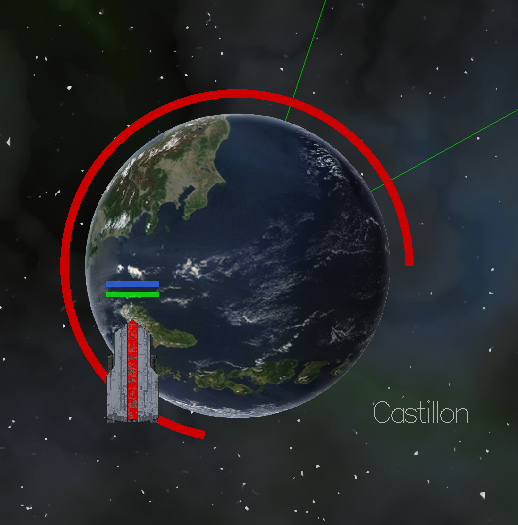
\includegraphics{res/planetary_capture}
	\caption[An example of planetary capture in Project Serenity]{The planet ``Castillon'' being captured by a red team ship}
	\label{fig:planetary-capture}
\end{marginfigure}

Every planet stores its current owner and the percentage by which it has been captured.
If the percentage captured is less than one hundred percent then the planet is said
to be partially captured. A planet's owner is the only player who is able to exploit
its resources. Figure~\ref{fig:planetary-capture} shows a planet that is approximately
seventy-five percent captured by a ship owned by the red player.

\vspace{-0.5em}
\begin{listing}{list:planetary-capture}{Mechanism of planetary capture}{Pseudocode for the mechanism of planetary capture}{}
\end{listing}\vspace{-1.5em}

\begin{tabbing}
$n \leftarrow$ number of different players with ships in vicinity of planet $p$ \\
{\bf if} $n = 1$ {\bf then} \\
\quad $o \leftarrow$ current owner of planet $p$ \\
\quad $a \leftarrow$ player with ships in the vicinty of planet $p$ \\
\quad $c \leftarrow$ percentage completion of planetary capture \\
\quad{\bf if} $o = a$ {\bf and} $c < 100$ {\bf then} \\
\quad\quad Increment the percentage captured by two \\
\quad{\bf elsif} $o \neq a$ {\bf and} $c > 0$ {\bf then} \\
\quad\quad Decrement the percentage captured by two \\
\quad{\bf elsif} $o \neq a$ {\bf then} \\
\quad\quad Change planet ownership from $o$ to $a$ \\
\quad\bf fi \\
\bf else \\
\quad $c \leftarrow$ percentage completion of planetary capture \\
\quad{\bf if} $c \leq 0$ {\bf then} \\
\quad\quad Reset the ownership of planet $p$ to nobody \\
\quad{\bf elsif} $c < 100$ {\bf then} \\
\quad\quad Decrement the percentage captured by one \\
\quad\bf fi \\
\bf fi
\end{tabbing}
\noindent
The full mechanism by which a planet, $p$, is shown in Listing~\ref{list:planetary-capture}.
If only a single player is in control of the area surrounding a planet then they either
increase the percentage by which it is captured if they are the current owner. If another
player is listed as the current owner then the percentage captured is decreased until it
reaches zero and ownership is transferred. However, if there are no players or multiple
players in the vicinity of a planet then the ownership of partially captured planets,
i.e. those that are not one hundered percent captured, starts to decay until it reaches
zero and the planet owner is reset.
